\textbf{Les questions 1, 2, 3 et 4 sont indépendantes.}

\subsection*{Question 1}
	On considère l'équation différentielle (E) :\quad  $y'=-2 y+90$ \quad où $y$ est une fonction définie sur $\R$ et $y'$ sa dérivée.

	\begin{enumerate}
		\item Déterminer l'ensemble des solutions de l'équation différentielle (E).
		\item Le plan est muni d'un repère orthonormé \Oij.

		Donner l'expression de la solution de (E) dont la courbe représentative dans ce repère passe par le point de coordonnées $(0 ; 30)$.
	\end{enumerate}



\subsection*{Question 2}
	Le cercle $C$ de centre 0 et de rayon 2 est représenté ci-dessous, dans le plan complexe muni d'un repère orthonormé \Ouv.

	Le point A d'abscisse 1 appartient au cercle $C$; on note $z_{\mathrm{A}}$ l'affixe du point A.

	\begin{center}
		\begin{center}
			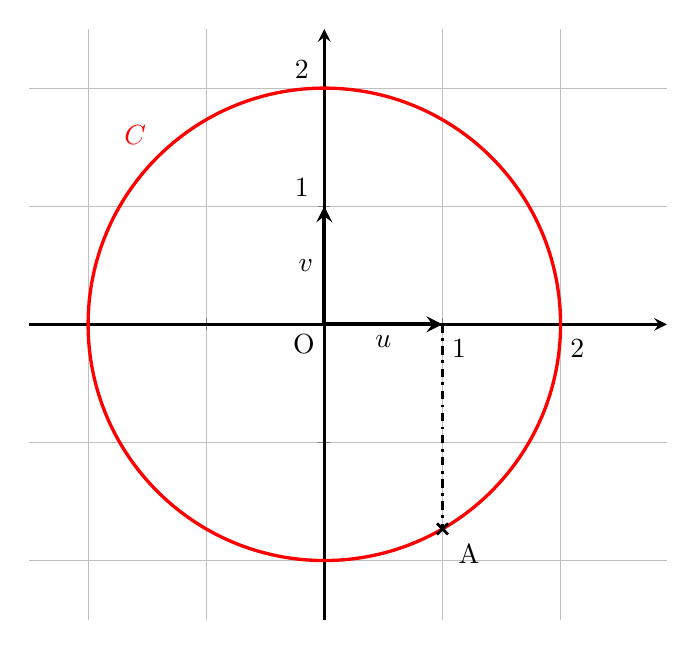
\begin{tikzpicture}[>=stealth]%compiler avec pgfplots
				\begin{axis}[/pgf/number format/.cd, use comma,
					x={15mm}, y={15mm},
					xmin = -2.5, xmax = 2.9,
					ymin = -2.5, ymax = 2.5,
					xtick distance=1,
					ytick distance=1,
					axis x line =middle, axis y line=middle,
					axis line style={line width=1pt},
					xticklabels={,,,,1,2,}, x tick label style={below right},
					yticklabels={,,,,1,2,}, y tick label style={above left},
					clip=false,
					,grid=major]
					tick label style={font=\footnotesize},
					minor tick num = 1,
					grid=major, axis lines =center]
					\node[below left] at (axis cs: 0,0) {O};
					\draw[line width=1.5pt,->] (axis cs: 0,0)-- (axis cs: 1,0)
					node[pos=0.5, below]{$\vect{u}$};
					\draw[line width=1.5pt,->] (axis cs: 0,0)-- (axis cs: 0,1)
					node[pos=0.5, left]{$\vect{v}$};
					\draw[red, line width=1.2pt] (axis cs: 0,0) circle (2) ;
					\node[red] at (axis cs: -1.6,1.6) {$C$};
					\draw[line width=1pt, dash dot] (axis cs: 1,0)--(axis cs: 1,-1.732);
					\draw[line width=1pt, shift={(axis cs: 1,-1.732)}]
					(2pt,2pt)--(-2pt,-2pt) (-2pt,2pt)--(2pt,-2pt) node[below right]{A};
				\end{axis}
			\end{tikzpicture}
		\end{center}

	\end{center}
	Donner la forme exponentielle de $z_{\mathrm{A}}$. Aucune justification n'est attendue.

\subsection*{Question 3}
	On considère la fonction $g$ définie sur $\R$ par :
	\[g(x)=\dfrac{x+2}{\e^{x}}\]

	\begin{enumerate}
		\item On note $g'$ la fonction dérivée de la fonction $g$. Montrer que pour tout $x$ réel,
		\[g'(x)=\dfrac{-1-x}{\e^{x}}\]

		\item En déduire les variations de la fonction $g$ sur $\R$.
	\end{enumerate}

\section*{Question 4}
	\begin{enumerate}
		\item Simplifier, en détaillant vos calculs, l'expression :
		\[\mathrm{A}=\ln \left(\dfrac{\e^{4}}{\e^{-2}}\right)\]

		\item Montrer, en détaillant vos calculs, que :
		\[\ln \left(\dfrac{9}{4}\right)+\ln \left(\dfrac{8}{3}\right)=\ln (6)\]
	\end{enumerate}
